\documentclass{beamer}

\usetheme{LMU}

\usepackage[utf8]{inputenc}
\usepackage[T1]{fontenc}

\usepackage[english]{babel}
\usepackage{url}
%\usepackage{cite}
%\usepackage{natbib}
\usepackage[backend=bibtex,style=authoryear,dashed=false]{biblatex}
\addbibresource{../bib/eigene.bib}
\addbibresource{../bib/itip-refs.bib}
\addbibresource{../bib/other-refs.bib}
\renewcommand{\bibfont}{\normalfont\scriptsize}
\setlength{\bibhang}{3ex}

\usepackage{amssymb, amsmath, amsfonts, enumerate}
%\usepackage{bbold}
\newcommand\hmmax{0}
\usepackage{bm}
%\usepackage{dsfont}
\usepackage{pxfonts}
\usepackage{xcolor}

\usepackage{tikz}
\usetikzlibrary{%
   arrows,%
   calc,%
   fit,%
   patterns,%
   plotmarks,%
   shapes.geometric,%
   shapes.misc,%
   shapes.symbols,%
   shapes.arrows,%
   shapes.callouts,%
   shapes.multipart,%
   shapes.gates.logic.US,%
   shapes.gates.logic.IEC,%
   er,%
   automata,%
   backgrounds,%
   chains,%
   topaths,%
   trees,%
   petri,%
   mindmap,%
   matrix,%
   calendar,%
   folding,%
   fadings,%
   through,%
   patterns,%
   positioning,%
   scopes,%
   decorations.fractals,%
   decorations.shapes,%
   decorations.text,%
   decorations.pathmorphing,%
   decorations.pathreplacing,%
   decorations.footprints,%
   decorations.markings,%
   shadows}
%\usepackage{bbold}
\usepackage{hyperref}

\setbeamertemplate{blocks}[rounded][shadow=true]
\definecolor{lmugreen2}{RGB}{0,120,94}
%\definecolor{lmugreen2}{RGB}{0,148,64}
\definecolor{lmugreen}{RGB}{0,140,84}
\definecolor{unidurham}{RGB}{126,49,123}

\parindent0pt
\setlength{\unitlength}{1ex}
\setlength{\fboxsep}{0ex}

\def\then{{\color{lmugreen}$\rule[0.35ex]{2ex}{0.5ex}\!\!\!\blacktriangleright$}}
%\def\then{{\color{lmugreen}$\blacktriangleright\!\blacktriangleright$}}
%\def\then{{\color{lmugreen}$\blacktriangleright$}}
%\def\then{{\color{lmugreen}$\Rrightarrow$}}
%\def\then{{\color{lmugreen}$\rhd$}}
%\def\then{{\color{lmugreen}$\gg\!\!\!\!\!\gg$}}
%\def\then{{\color{lmugreen}${\mathbf{\gg}}$}}
\def\play{{\color{lmugreen}$\blacktriangleright$}}

\def\rthen{{\color{lmugreen}$\rule[0.35ex]{0.5ex}{0.95ex}\rule[0.35ex]{1.3ex}{0.5ex}\!\!\!\blacktriangleright$}}

\def\thenthen{{\color{lmugreen}$\blacktriangleleft\!\!\!\rule[0.35ex]{2ex}{0.5ex}\!\!\!\blacktriangleright$}}

\def\gplus{{\color{lmugreen}\rule[0.45ex]{1.4ex}{0.4ex}\hspace{-0.9ex}\rule[0.0ex]{0.4ex}{1.3ex}\hspace{0.5ex}}}
\def\gminus{{\color{lmugreen}\rule[0.45ex]{1.4ex}{0.4ex}}}


\def\blau#1{{\color{lmugreen2}#1}}
\def\rot#1{{\color{red}#1}}
\def\gruen#1{{\color{blue}#1}}
%\def\gruen#1{{\color{gray}#1}}

%%%%%%%%%%%%%%%%%%%%%%%%%%%%%%%%%%%%%%%%%
%% Definitions & shortcuts for thesis  %%
%%%%%%%%%%%%%%%%%%%%%%%%%%%%%%%%%%%%%%%%%

\def\pdc{prior-data conflict}

\newcommand{\reals}{\mathbb{R}}

\newcommand{\dd}{\,\mathrm{d}}

\newcommand{\mbf}[1]{\mathbf{#1}}

\newcommand{\X}{\mbf{X}}
\newcommand{\x}{\mbf{x}}

\def\yzr{\rot{\yz}}
\def\ynr{\rot{\yn}}
\def\byzr{\rot{\byz}}
\def\bynr{\rot{\byn}}
\def\yzor{\rot{y\uz_1}}
\def\yzjr{\rot{y\uz_j}}
\def\yzkr{\rot{y\uz_k}}
\def\yzlr{\rot{\yzl}}
\def\yzur{\rot{\yzu}}
\def\ynjr{\rot{y\un_j}}
\def\ynlr{\rot{\ynl}}
\def\ynur{\rot{\ynu}}
\def\yzjlr#1{\rot{\ul{y}\uz_#1}}
\def\yzjur#1{\rot{\ol{y}\uz_#1}}


\def\nzg{\gruen{\nz}}
\def\nng{\gruen{\nn}}
\def\nzlg{\gruen{\nzl}}
\def\nzug{\gruen{\nzu}}
\def\nnlg{\gruen{\nnl}}
\def\nnug{\gruen{\nnu}}

\def\psib{\blau{\psi}}
\def\bpsib{\blau{{b}(\psi)}}


% ------------ shading start
\newsavebox{\tempbox}
\newcommand\leftrightshading[3]{%
  \begin{tikzfadingfrompicture}[name=inputtext]
    \node [text=white] {#1};
  \end{tikzfadingfrompicture}
  \begin{lrbox}{\tempbox}%
    \begin{tikzpicture}
      \node [text=white,inner sep=0pt,outer sep=0pt] (textnode) {#1};
      \shade[path fading=inputtext,fit fading=false,left color=#2,right color=#3]
      (textnode.south west) rectangle (textnode.north east);
    \end{tikzpicture}%
  \end{lrbox}
  % Now we use the fading in another picture:
  \usebox\tempbox{}%
}
% ------------ shading end


%\def\PZc{\mathrm I\!\Pi\uz}
\def\PZc{\leftrightshading{$\mathrm I\!\Pi\uz$}{blue}{red}}
%\def\PNc{\PN}
\def\PNc{\leftrightshading{$\mathrm I\!\Pi\un$}{blue}{red}}


\title[Generalised Bayesian Inference \& Prior-Data Conflict]
{Generalised Bayesian Inference\\ under Prior-Data Conflict}

\author%[]
       {Gero Walter}

\institute{Department of Statistics\\
           Ludwig-Maximilians-Universit\"at M\"unchen (LMU)\\
                      {}%\{gero.walter; thomas\}@stat.uni-muenchen.de
}

\date{October 25th, 2013}


\titlegraphic{
%\begin{center}

\includegraphics[scale=0.032]{lmu_logos/lmu_massiv.png}
\raisebox{1.375cm}{
\includegraphics[scale=0.4]{lmu_logos/lmu_statistic.pdf}
}
%\end{center}
}

%---- Notes ---------------------
\setbeameroption{hide notes}
%\setbeameroption{show only notes}

\begin{document}


\frame{
\titlepage
}

\frame{\frametitle{Overview}
\begin{tikzpicture}
\node[draw] at (0,0) {\includegraphics[scale=0.25]{../diss-toc-1.pdf}};
%\draw[decorate,decoration={brace,mirror,raise=5pt},blue]
\draw[thick,decorate,decoration=brace] (2.2,-1.5) -- (2.2,-2.7) node[midway,right,align=left] %
{motivating example:\\ {\color{lmugreen} common-cause failure}};
\end{tikzpicture}
}

\frame{\frametitle{Overview}
\begin{enumerate}
\item Introduction
 \begin{enumerate}
 \item Preliminaries
 \item Some Fundamentals
 \item Dirichlet-Multinomial Model for Common-Cause Failure
 \end{enumerate}
\item Imprecise Probability as Foundation of Generalised Bayesian Inference
 \begin{enumerate}
 \item Imprecise or Interval Probability
 \item Motives for the Use of Imprecise Probability
 \end{enumerate}
\item Generalised Bayesian Inference with Sets of Conjugate Priors in Exponential Families
 \begin{enumerate}
 \item Model Overview and Discussion
 \item Alternative Models Using Sets of Priors
 \item Imprecision and Prior-Data Conflict in Generalised Bayesian Inference
 \item The \texttt{luck} Package
 \item On Prior-Data Conflict inPredictive Bernoulli Inferences
 \end{enumerate}
\end{enumerate}
}

\frame{\frametitle{Overview}
\begin{enumerate}
\item[4.] Concluding Remarks
 \begin{enumerate}
 \item[4.1] Summary
 \item[4.2] Discussion
 \item[4.3] Outlook
 \end{enumerate}
\item[A.] Appendix
 \begin{enumerate}
 \item[A.1] Bayesian Linear Regression: Different Conjugate Models and Their (In)Sensitivity to Prior-Data Conflict
 \item[A.2] A Parameter Set Shape for Strong Prior-Data Agreement Modelling
 \end{enumerate}
\end{enumerate}

Outline of the talk***
\begin{enumerate}
\item Common-cause failure modelling\\ (joint work with Matthias Troffaes and Dana Kelly)
\item Generalised Bayesian inference with sets of priors\\ (joint work with Thomas Augustin)
\item Prior-data conflict and Strong prior-data agreement\\ (joint work with Thomas Augustin and Frank Coolen)
\end{enumerate}

}

\section{Common-cause Failure Modelling}


\frame{\frametitle{Common-Cause Failures}
\begin{tikzpicture}
\uncover<1->{
\node {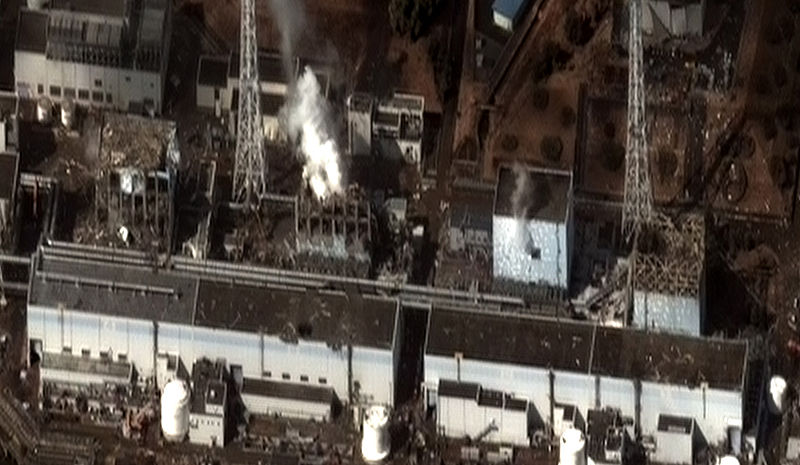
\includegraphics[scale=0.4]{./graph/800px-Fukushima_I_by_Digital_Globe.jpg}};
\node at (0,-3.5) {\tiny Source: Wikimedia Commons, \url{http://commons.wikimedia.org/wiki/File:Fukushima_I_by_Digital_Globe.jpg}};
}
\uncover<2->{
%\draw[white,fill=white] (-5,1) rectangle (5,3);
\node at (0,2.6) {\parbox{\textwidth}{
 \begin{alertblock}{common-cause failure} 
 \emph{simultaneous failure of several redundant components\\ due to a common or shared root cause}
 (H{\o}yland \& Rausand, 1994)
 \end{alertblock}
}};
}
\uncover<3>{
\draw[white,fill=white] (-0.2,-3.3) rectangle (6,0.75);
\node at (3,-1) {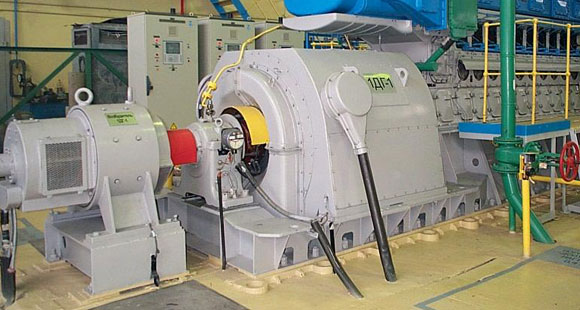
\includegraphics[scale=0.3]{./graph/plant-systems-diesel-generator.jpg}};
\node at (3.05,-3.05) {\parbox{6.2cm}{\tiny Source: \url{http://www.diakont.com/solutions/nuclear-energy/plant-systems/diesel-generator-control-systems/}}};
}
\end{tikzpicture}

% Notes for the slide
\note<3>[item]{All 12 generators (for 6 reactors) at Fukushima Daiichi\\ were not available due to flooding of machine rooms\\
 (Tsunami caused by T\={o}hoku earthquake)}
\note<3>[item]{Reliability of redundant systems}
\note<3>[item]{Usually 2 -- 4 emergency diesel generators per reactor}
\note<3>[item]{Sufficient cooling of core if one generator works}
\note<3>[item]{Reliability through redundancy is jeopardised by common-cause failure:}
\note<3>[item]{Redundant components may not fail independently: common-cause failure}
\note<3>[item]{Must include common-cause failures in overall system reliability analysis}
}

\frame{
\frametitle{Common-Cause Failure Modelling ***raus?}

\begin{columns}%[T]
\begin{column}{0.7\textwidth}\centering
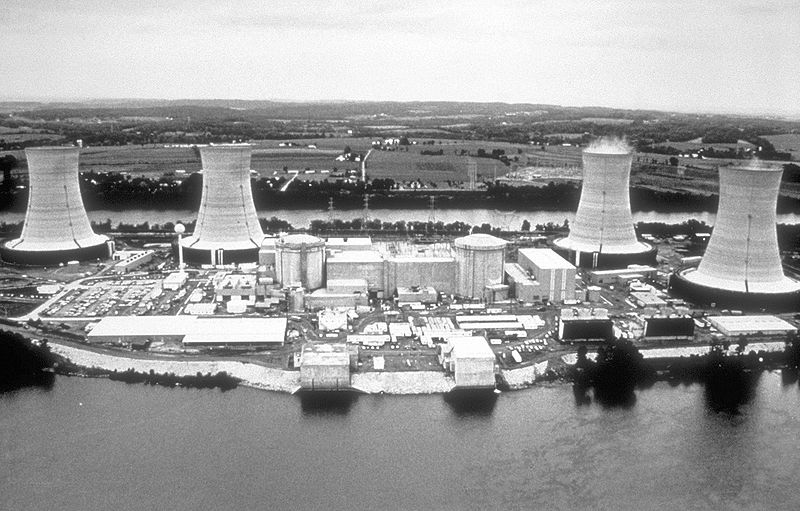
\includegraphics[scale=1.2]{./graph/800px-Three_Mile_Island_nuclear_power_plant.jpg}
\end{column}
\begin{column}{0.35\textwidth}\centering
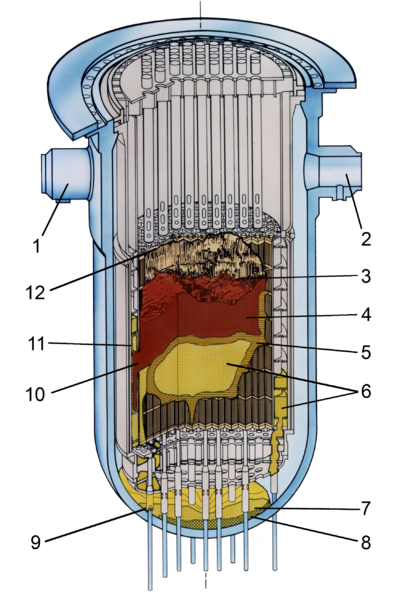
\includegraphics[scale=0.95]{./graph/Graphic_TMI-2_Core_End-State_Configuration.png}
\end{column}
\end{columns}
\vspace*{1ex}
\begin{tiny}
Above: CDC, \url{http://phil.cdc.gov/phil/} ID 1194\\[1ex]
Right: Wikimedia Commons,\\[-1.8ex]
\url{http://commons.wikimedia.org/wiki/File:Graphic_TMI-2_Core_End-State_Configuration.png}
\end{tiny}
% Notes for the slide
\note<1>[item]{Lesson learned at another accident: Three Mile Island (1979) where also a meltdown happened (right)}
\note<1>[item]{Most popular model: \emph{basic parameter model}, we will look at a parameterisation of it called\ldots}
}

\subsection{Alpha-Factor Model}

\begin{frame}{Alpha-Factor Model: Definition}
  \begin{block}{Alpha-Factor Model} %\cite{1988:mosleh::common:cause}]
    Multinomial distribution $\mult(\vec{n}\mid\vec{\alpha})$ for common-cause failures \\
    in a $k$-component system\vspace*{-2ex}
    %the number of redundant components in the common-cause component group
    \begin{align*}
      p(\vec{n}\mid\vec{\alpha})=\prod_{j=1}^k\alpha_j^{n_j}\\[-5ex]
    \end{align*}
    where
    \begin{itemize}
    \item \alert{alpha-factor}
      $\alpha_j\coloneqq$
      \parbox[t]{0.6\textwidth}{%
        probability of $j$ of the $k$ components \\
        failing due to a common cause \\
        given that failure occurs
      }
    \item \alert{failure count}
      $n_j\coloneqq$ corresponding number of failures observed
    \item $\vec{n}$ denotes $(n_1,\dots,n_k)$ and $\vec{\alpha}$ denotes $(\alpha_1,\dots,\alpha_k)$
    \end{itemize}
  \end{block}
  (the model actually serves to estimate failure \emph{rates},\\ but the above is all what matters in this talk)
\end{frame}

\iffalse
\begin{frame}{Alpha-Factor Model: Inference ***raus??***}
  \begin{block}{Inference}
    involves rational functions \\
    of probabilities $\vec{\alpha}$ of common-cause failures\\
    and of total failure rate $q_t$ for individual components
  \end{block}
  \begin{center}
    \textbf{this talk: focus on $\vec{\alpha}$ only}
  \end{center}
\end{frame}
\fi

\begin{frame}{Alpha-Factor Model: Parameter Estimation}
\uncover<1->{%
  \begin{exampleblock}{The Good News}
    attractive feature of this model: \\
    $\vec{\alpha}$ can be estimated directly from data, e.g.\ MLE:
    \begin{align*}
      \alpha_j &= \frac{n_j}{n},\quad \text{where $\textstyle\sum_{j=1}^n n_j = n$}
    \end{align*}
  \end{exampleblock}}
\uncover<2->{%
  \begin{alertblock}{The Bad News}
    \begin{itemize}
    \item typically, for $j\ge 2$, the $n_j$ are very low \\
      with zero being quite common for larger $j$
    \item zero counts = flat likelihoods \\
      standard techniques such as MLE can struggle \\
      to produce sensible inferences for this problem
    \end{itemize}
  \end{alertblock}}
\uncover<3>{%
  \vspace*{-1ex}
  \begin{center}
    \textbf{\then\ need to rely on \alert{epistemic information}}
  \end{center}}
\end{frame}

\frame{\frametitle{References}

\nocite{Walter2009a-short,1994:hoyland,1965:good,1991:walley,1996:walley::idm,2011:kelly:atwood,1996:atwood,Troffaes2013a-short,2006:evans,2005:quaeghebeurcooman-short}

\printbibliography[heading=none]

%\bibliographystyle{plainnat}
%\bibliography{../bib/eigene,../bib/itip-refs,../bib/other-refs}
}



%---- Appendix: Updating and Mixture Commute

\frame{\frametitle{Updating and Mixture Commute}

Let
\begin{align*}
p_m(\vartheta\mid \nz_1\!,\yz_1\!, \nz_2\!,\yz_2\!, \kappa) &:=
   \kappa\,  p(\vartheta\mid\nz_1\!,\yz_1) +
(1-\kappa)\, p(\vartheta\mid\nz_2\!,\yz_2) \,,
\end{align*}
with marginals
\begin{align*}
f_1(\x) &= \int_\Theta\! f(\x\mid\vartheta) p(\vartheta\mid \nz_1\!,\yz_1) \dd\vartheta \,, \\
f_2(\x) &= \int_\Theta\! f(\x\mid\vartheta) p(\vartheta\mid \nz_2\!,\yz_2) \dd\vartheta \,, \\
f_m(\x) &= \int_\Theta\! f(\x\mid\vartheta) p_m(\vartheta\mid \nz_1\!,\yz_1\!, \nz_2\!,\yz_2\!, \kappa) \dd\vartheta \\
        &=    \kappa  \int_\Theta f(\x\mid\vartheta) p(\vartheta\mid \nz_1\!,\yz_1) \dd\vartheta 
         + (1-\kappa) \int_\Theta f(\x\mid\vartheta) p(\vartheta\mid \nz_2\!,\yz_2) \dd\vartheta \\
%        &=    \kappa  \int_\Theta f_1(\x) p(\vartheta\mid \nn_1,\yn_1) \dd\vartheta 
%         + (1-\kappa) \int_\Theta f_2(\x) p(\vartheta\mid \nn_2,\yn_2) \dd\vartheta \\
        &= \kappa f_1(\x) + (1-\kappa) f_2(\x) \,.
\end{align*}

}

\frame{\frametitle{Updating and Mixture Commute}

%Then
\begin{align*}
\lefteqn{
p_m(\vartheta\mid \nz_1,\yz_1, \nz_2,\yz_2, \kappa, \x) } \hspace*{8ex} & \\[2ex]
 &= \frac{f(\x\mid\vartheta)}{f_m(\x)} \big(
     \kappa\,  p(\vartheta\mid\nz_1,\yz_1) +
  (1-\kappa)\, p(\vartheta\mid\nz_2,\yz_2) \big) \\
 &=  \kappa\,  \frac{f(\x\mid\vartheta) p(\vartheta\mid\nz_1,\yz_1)}{f_m(\x)} +
  (1-\kappa)\, \frac{f(\x\mid\vartheta) p(\vartheta\mid\nz_2,\yz_2)}{f_m(\x)} \\
 &=  \kappa\,  \frac{f_1(\x) p(\vartheta\mid\nn_1,\yn_1)}{f_m(\x)} +
  (1-\kappa)\, \frac{f_2(\x) p(\vartheta\mid\nn_2,\yn_2)}{f_m(\x)} \\
 &= p_m(\vartheta\mid \nn_1,\yn_1, \nn_2,\yn_2, \kappa^*)\,,
\end{align*}
\begin{align*}
\text{where}\hspace{5ex}
\kappa^* &= \kappa\, \frac{f_1(\x)}{f_m(\x)}
          = \frac{\kappa\, f_1(\x)}{\kappa\, f_1(\x) + (1-\kappa)\, f_2(\x)}\,. 
\end{align*}

}

\frame{\frametitle{Updating and Mixture Commute}

\begin{itemize}
\item updated mixture distribution is a mixture of the updated components
with mixture parameter $\kappa^*$ instead of $\kappa$.
\item convex hull of prior components\\ $=$ set of prior mixture distributions with $\kappa \in [0,1]$
\item for any $\kappa \in [0,1]$, the corresponding $\kappa^* \in [0,1]$.
\item in fact, $\{\kappa^* \mid \kappa \in [0,1]\} = [0,1]$.
\item set of updated mixture distributions with $\kappa^* \in [0,1]$\\ $=$ convex hull of updated components
\item arbitrary number of components by complete induction
\end{itemize}
}


%---- Appendix: reset frame number
\addtocounter{framenumber}{-3} 

\end{document}
